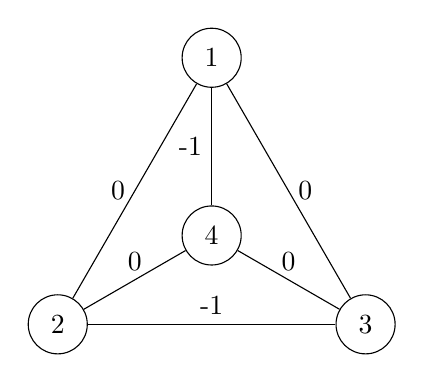
\begin{tikzpicture}
\node[circle,minimum size=4.5 cm,overlay] (b) {};
\foreach\x in{1,...,3}{
  \node[minimum size=0.75cm,draw,circle] (\x) at (b.{120*\x-30}){\x};
}
\node[minimum size=0.75cm,draw,circle] (4) at (0,0) {4};

\draw (1) -- (2) node [midway, above, left] {0};
\draw (1) -- (3) node [midway, above, right] {0};
\draw (1) -- (4) node [midway, left] {-1};
\draw (2) -- (3) node [midway, above] {-1};
\draw (2) -- (4) node [midway, above] {0};
\draw (3) -- (4) node [midway, above] {0};

\end{tikzpicture}